
\subsection{RQ1: Evaluation of existing history generation tools}

% \subsubsection{Motivation}
% Reliable method-level revision histories are fundamental to empirical studies of software evolution and maintenance. In this study, such histories are necessary to characterize the evolution of test methods with respect to their corresponding methods under test, investigate test--production co-evolution, and identify test methods that are recurrently revision-prone. Incomplete histories may omit relevant test changes, whereas incorrect histories may attribute unrelated changes to a test method; both cases can bias downstream findings. Although existing tools can generate method-level histories, they were primarily designed and evaluated for production methods. Consequently, it remains unclear whether they can recover test-method histories accurately.

% Recovering test-method histories can be particularly challenging because test classes and methods often follow naming conventions derived from the corresponding production class or method. For example, developers may add a conventional \texttt{test} prefix or suffix to the class name, the method name, or both. As a result, a test method and its associated production method may appear similar under name-based or similarity-based matching heuristics, increasing the risk that a tool follows the wrong lineage.

%For example, Commons Lang contains the test method
%\texttt{testToCharArray} in
%\texttt{StrBuilderTest}\footnote{\href{https://github.com/apache/commons-lang/blob/7bcb03a49923bc12f7e3f2c04912d0925f178978/src/test/java/org/apache/commons/lang3/text/StrBuilderTest.java\#L1741}{GitHub source}}
%and the production method \texttt{toCharArray} in
%\texttt{StrBuilder}\footnote{\href{https://github.com/apache/commons-lang/blob/7bcb03a49923bc12f7e3f2c04912d0925f178978/src/main/java/org/apache/commons/lang3/text/StrBuilder.java\#L2949}{GitHub source}}
%in the same package.  The class names differ only by the \texttt{Test} suffix,
%while the method names differ only by the \texttt{test} prefix.
%
%This risk occurred during our oracle construction.  While tracing a selected
%test method in
%\texttt{TestCheckpoint}\footnote{\href{https://github.com/apache/hadoop/blob/c6e716bf5bc8958a1f5fc63d1b2844a2f8f118be/hadoop-hdfs-project/hadoop-hdfs/src/test/java/org/apache/hadoop/hdfs/server/namenode/TestCheckpoint.java\#L1967}{GitHub source}},
%HistoryFinder incorrectly mapped the lineage through another test method and
%then followed the production method \texttt{create} in
%\texttt{FTPFileSystem}\footnote{\href{https://github.com/apache/hadoop/blob/c6e716bf5bc8958a1f5fc63d1b2844a2f8f118be/hadoop-common-project/hadoop-common/src/main/java/org/apache/hadoop/fs/ftp/FTPFileSystem.java\#L313}{GitHub source}},
%resulting in four false-positive commits.  Since existing method-history tools
%have mainly been evaluated on production methods
%\cite{grund:2021,jodavi_accurate_2022,islam_historyfinder_2025}, their
%effectiveness for test-method history generation requires a dedicated
%evaluation.

To advance research on test code evolution, it is necessary to determine whether tools developed for production code generalize to test code or require retraining and threshold recalibration.
\subsubsection{Approach}
The \emph{CodeShovel}~\cite{grund:2021} and \emph{CodeTracker}~\cite{jodavi_accurate_2022} studies used the same 20 popular open-source Java projects to construct their evaluation oracles. \emph{HistoryFinder}~\cite{islam_historyfinder_2025} later expanded this benchmark by adding 20 additional projects. All 40 projects were used to construct a new oracle for evaluating test-method history generation. From each project, three test methods were randomly selected, resulting in 120 test-method histories, slightly more than the original \emph{CodeShovel}~\cite{grund:2021} study, which used 100 methods as test data.

To construct the ground truth, the methodology of \emph{HistoryFinder}~\cite{islam_historyfinder_2025} was followed. Specifically, candidate change commits were collected from six history-generation tools: \emph{HistoryFinder}, \emph{CodeShovel}, \emph{CodeTracker}, \emph{IntelliJ}, \emph{GitLineRange}, and \emph{GitFuncName}. The union of all commits reported by these tools was then formed, which offers almost perfect recall~\cite{islam_historyfinder_2025}, but contains many false positives. This is why, similar to ~\cite{islam_historyfinder_2025}, the first and second authors, graduate students in software engineering with over 10 years and 1 year of industry experience, respectively, independently reviewed each of the generated commits to filter out the false positives, requiring $\approx$80 person-hours. The agreement score was near perfect (Cohen's Kappa of 0.98). The disagreements in 10 commits were subsequently resolved through in-person discussion. Following prior studies~\cite{grund:2021,islam_historyfinder_2025}, any selected test method with fewer than three revisions was replaced by another randomly selected test method from the same project with at least three revisions.


Similar to \emph{HistoryFinder}~\cite{islam_historyfinder_2025}, the tools' performance was assessed at both the commit and method levels. At the commit level, true positives, false positives, and false negatives were aggregated across all test methods before computing precision, recall, and F1 score. At the method level, these metrics were computed separately for each test method and their averages were reported. The execution time (the average of five runs) required to generate each method history was also measured. Experiments were conducted on a machine running Ubuntu 22.04 LTS with 32 GB of RAM, an Intel(R) Core(TM) i7-8700 CPU @ 3.20 GHz (12 cores), and Java 21 (x86). To avoid cross-run caching effects, each tool was executed independently for every method. Similar to~\cite{islam_historyfinder_2025}, \emph{IntelliJ} was excluded from the runtime comparison because its histories must be obtained manually through the IDE's built-in history-tracking feature.

\subsubsection{Result}
\begin{table*}[htbp]
\centering
\caption{Accuracy of the method-history tracking tools. \textbf{TP} denotes correctly identified change commits, \textbf{FP} denotes incorrectly included commits, and \textbf{FN} denotes missed change commits.}
\label{tab:t2p-method-tracking-score}
\begin{tabular}{lrrrrrrrrr}
\toprule
\multirow{2}{*}{\textbf{Tool}} &
\multicolumn{6}{c}{\textbf{\emph{Commit-Level}}} &
\multicolumn{3}{c}{\textbf{\emph{Method-Level}}} \\
\cmidrule(lr){2-7} \cmidrule(lr){8-10}
& \textbf{TP} & \textbf{FP} & \textbf{FN} &
\textbf{Precision} & \textbf{Recall} & \textbf{F1} &
\textbf{Precision} & \textbf{Recall} & \textbf{F1} \\
\midrule
CodeShovel    & 644          & \textbf{3} & 16         & \textbf{99.54} & 97.58          & 98.55          & 99.35          & 97.82          & 98.27 \\
CodeTracker   & 667          & 11         & 18         & 98.38          & 97.37          & 97.87          & 97.56          & 96.57          & 97.72 \\
HistoryFinder & \textbf{721} & 5          & \textbf{1} & 99.31          & \textbf{99.86} & \textbf{99.59} & \textbf{99.63} & \textbf{99.65} & \textbf{99.60} \\
IntelliJ      & 549          & 180        & 171        & 75.31          & 76.25          & 75.78          & 87.90          & 76.96          & 79.72 \\
GitLineRange  & 343          & 58         & 350        & 85.54          & 49.49          & 62.71          & 92.56          & 51.40          & 61.80 \\
GitFuncName   & 86           & 8          & 611        & 91.49          & 12.34          & 21.74          & 98.90          & 10.69          & 11.35 \\
\bottomrule
\end{tabular}


\end{table*}


Table~\ref{tab:t2p-method-tracking-score} shows that all three research-based tools substantially outperform the \emph{IntelliJ} and \emph{Git-based} baselines. At the commit level, \emph{HistoryFinder} achieves the best overall accuracy, attaining the highest recall (99.86\%) and F1 score (99.59\%). \emph{CodeShovel} achieves the highest precision (99.54\%) and also performs strongly overall, with an F1 score of 98.55\%. \emph{CodeTracker} follows closely with an F1 score of 97.87\%. The method-level results exhibit a similar trend.

Table~\ref{tab:method-history-runtime} and Figure~\ref{fig:method-history-runtime-boxplot} compare the runtime performance of these tools. The \emph{Git-based} approaches achieve the lowest runtimes; however, this advantage largely stems from terminating history tracing much earlier than the other tools, resulting in substantially lower recall. Among the research-based approaches, \emph{HistoryFinder} is the most efficient, with the lowest mean (1.47 seconds) and median (0.63 seconds) runtimes. \emph{CodeTracker} exhibits the greatest runtime variability and the highest maximum runtime (943.93 seconds), primarily due to its reliance on \emph{RefactoringMiner}~\cite{tsantalis2020refactoringminer} for tracking refactorings. In contrast, both \emph{HistoryFinder} and \emph{CodeShovel} rely on lightweight string-based similarity techniques, resulting in lower and more stable runtimes.


\begin{table}[htbp]
\centering
\caption{Runtime of the history generation tools in seconds.}
\label{tab:method-history-runtime}
\begin{tabular}{lrrr}
\toprule
\textbf{Tool} & \textbf{Mean} & \textbf{Median} & \textbf{Max} \\
\midrule
HistoryFinder & 1.47 & 0.63 & 37.87 \\
CodeShovel & 2.52 & 1.22 & 42.02 \\
CodeTracker & 26.53 & 1.14 & 943.93 \\
GitLineRange & 1.18 & 0.28 & 20.81 \\
GitFuncName & \textbf{0.32} & \textbf{0.18} & \textbf{3.95} \\
\bottomrule
\end{tabular}


\end{table}

\begin{figure}[htbp]
\setlength{\belowcaptionskip}{-10pt}

    \centering
    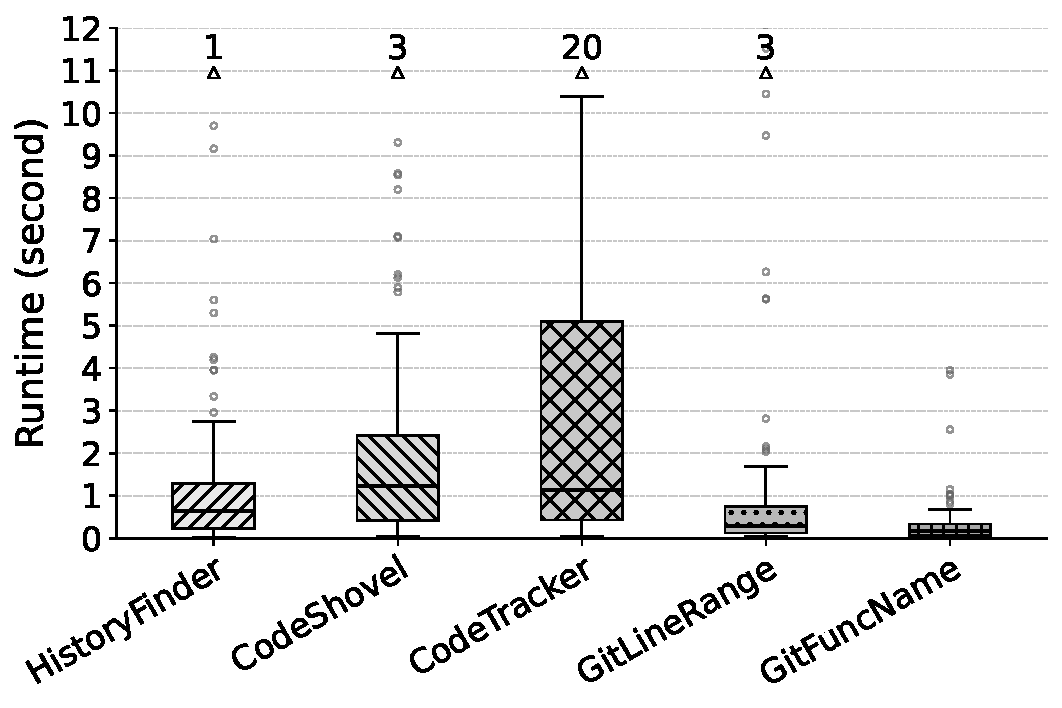
\includegraphics[width=0.8\columnwidth,keepaspectratio]{figure/method-history-runtime-boxplot.pdf}
    \caption{Runtime of the studied tools. The y-axis is capped at 12s for readability; triangles indicate values above the limit, with numbers showing their counts.}
    \label{fig:method-history-runtime-boxplot}
\end{figure}

\begin{tcolorbox}
\noindent\textbf{\underline{RQ1 summary}:}
Considering both accuracy and runtime, \emph{HistoryFinder} is the best tool for tracking test method change history. Overall, the results are encouraging, as they suggest researchers can use existing tools directly without the cost of retraining them for test methods.
\end{tcolorbox}
